\renewcommand*{\arraystretch}{1.1}

\label{sec:interactive-update-03}
\noindent\begin{tabularx}{\queryCardWidth}{|>{\queryPropertyCell}c|X|}
	\hline
	query & Interactive / update / 3 \\ \hline
%
	title & Add Comment Like \\ \hline
%
    pattern & \hfill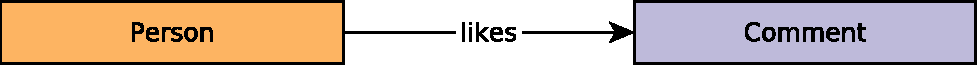
\includegraphics[scale=\patternscale,margin=0cm .2cm]{patterns/interactive-update-03}\hfill\vadjust{} \\ \hline
%
	desc. & Add a Like to a Comment of the social network.
 \\ \hline
%
	
%
    
        params &
        \innerCardVSpace{\begin{tabularx}{\attributeCardWidth}{|>{\paramNumberCell}c|>{\varNameCell}M|>{\typeCell}m{\typeWidth}|Y|} \hline
        \cellcolor{parameter} \color{white} \footnotesize $\mathsf{1}$ &Person.id& ID &  \\ \hline
        \cellcolor{parameter} \color{white} \footnotesize $\mathsf{2}$ &Comment.id& ID &  \\ \hline
        \cellcolor{parameter} \color{white} \footnotesize $\mathsf{3}$ &Person-likes->.creationDate& DateTime &  \\ \hline
        \end{tabularx}}\innerCardVSpace \\ \hline
	
%
	
%
	%
	%
	%
    %
\end{tabularx}
\queryCardVSpace